\documentclass{book}
\usepackage[utf8]{inputenc}
\usepackage[english]{babel}
\usepackage[fleqn]{amsmath}
\usepackage{amssymb}
\usepackage{parskip} % turns off the indentation and adds a little bit of (stretchable) space in between paragraphs.
\usepackage{graphicx}
\usepackage{wrapfig}

\graphicspath{ {images/} }

\DeclareMathOperator\cis{cis} % used for complex numbers
 % most of the time, \newcommand* is the best choice as you want the error-checking that it provides.
\newcommand*\conj[1]{\bar{#1}}
\newcommand*\mean[1]{\bar{#1}}
\newcommand*\reciprocal[1]{\frac{1}{#1}}
\newcommand*\argument{\phi}

% number sets
\newcommand*\primes{\mathbb{P}}
\newcommand*\naturalnumbers{\mathbb{N}}
\newcommand*\wholenumbers{\mathbb{W}}
\newcommand*\integers{\mathbb{Z}}
\newcommand*\rationalnumbers{\mathbb{Q}}
\newcommand*\irrationalnumbers{\mathbb{I}}
\newcommand*\reals{\mathbb{R}}
\newcommand*\complexnumbers{\mathbb{C}}

\title{Formulas}
\author{Bernardo Sulzbach}
\date{October 2015}

\begin{document}

\maketitle

\chapter{Introduction}
This document is a collection of notes and formulas from various subjects I
need to remember. It is mainly for reference purposes.

\chapter{Chemistry}

Ideal gas law
\[PV = nRT\]

Diffusion. Diffusion is the rate at which two gases mix.
Effusion. Effusion is the rate at which a gas escapes through a pin hole.

Graham's law of diffusion or effusion

Graham's law states that the rate of effusion or of diffusion of a gas is
inversely proportional to the square root of its molecular weight.

\[\frac{R_1}{R_2} = \sqrt{\frac{M_2}{M_1}}\]

In the same conditions of temperature and pressure, the molar mass is
proportional to the mass density. Therefore the rate of diffusion of different
gases is inversely proportional to the square root of their mass densities.

\[\frac{R_1}{R_2} = \sqrt{\frac{M_2}{M_1}}\]

Solution. A solution is a homogeneous mixture of two or more substances.

Solute is a substance that is dissolved in the solution.

Solvent is the substance that dissolves the solute. Solvent is present in
greater amount.

Concentration is the ratio of solute and solvent.

Concentration can be measured using molarity, molality and mole fraction.

\[\text{Molarity (M)} = \frac{\text{moles of solute}}{\text{liters of solution}}\]

\[\text{Molality (m)} = \frac{\text{moles of solute}}{\text{kg of solution}}\]

Mole fraction. The mole fraction of a component in solution is the number of
moles of that component divided by the total number of moles of all components
in the solution.

\[X_A = \frac{n_A}{\sum{n_x}}\]

Dilution. Diluting a solution means adding more solvent without adding more solute.
The following formula is quite helpful in these calculations.

\[M_i V_i = M_f V_f\]

Mole. Mole is the amount of substance that contains same number of particles as
there are atoms in 12 grams of pure carbon-12.

One mole of substance is Avogadro's number.

The number of molecules in a mole is known as Avogadro's constant.

\[N_A = 6.023 \cdot 10^{23}\]

One mole of gas has a volume of 22.4 liters at Standard Temperature and Pressure.

Relation between moles and grams.
One mole of a substance weights the molecular weight of substance in grams.

Ionization energy. Ionization energy is qualitatively defined as the amount of
energy required to remove the most loosely bound electron of an isolated
gaseous atom to form a cation. It is always endothermic (positive).

The Henderson-Hasselbalch equation describes the derivation of pH as a
measure of acidity (using pKa, the negative log of the acid dissociation
constant).

\[pH = pK_a + \log_{10} \frac{[\text{A}^-]}{[\text{HA}]}\]
\[pOH = pK_b + \log_{10} \frac{[\text{BH}^+]}{[\text{B}]}\]

where [A-] is the concentration of conjugate base and [HA] is the concentration
of the acid.


\chapter{Physics}

\section{Kinetics}
\[S = S_0 + V_0 t + \frac{a t^2}{2}\]
\[V_f^2 = V_i^2 + 2 a \Delta S\]

\section{Waves}
\[v = \lambda f\]

\subsection{Doppler Effect}
\[f = f_0 \left ( \frac{v + v_r}{v + v_s} \right )\]

where

\(v\) is the velocity of waves in the medium;

\(v_r\) is the velocity of the receiver relative to the medium; positive if the
receiver is moving towards the source (and negative in the other direction);

\(v_s\) is the velocity of the source relative to the medium; positive if the
source is moving away from the receiver (and negative in the other direction).

One can remember that the velocities are positive if the receiver is chasing
the source.

\section{Gases}
\[P = P_A + \rho g h\]
\[\tau = P \Delta V\]

\section{Electricity}
\[U = R i\]
\[P = i U\]
Resistance of a parallel association of resistors:
\[\reciprocal{R_{eq}} = \sum{\reciprocal{R_i}}\]

\subsection{Electric Force}
\[F_{el} = \frac{k Q q}{r^2}\]
\section{Electromagnetism}

\subsection{Magnetic Force}
\[F_{mag} = B q v = B i l\]

\subsection{Magnetic Fields}
\[B_{\text{wire}} = \frac{i \mu_0}{2 \pi r}\]
\[B_{\text{current loop}} = \frac{i \mu_0}{2 r}\]

\section{Modern Physics}
\[E = hf = h\frac{c}{\lambda}\]

\subsection{Lorentz factor}
The Lorentz factor is the factor by which time, length, and relativistic mass
change for an object while that object is moving.
\[\gamma = \reciprocal{\sqrt{1 - \frac{v^2}{c^2}}}\]

\chapter{Mathematics}

\section{Complex numbers}

\subsection{Notation}
\[\cis \left ( \argument \right ) =  \cos \left ( \argument \right ) + i \sin \left ( \argument \right )\]

\subsection{Formulas}
\[a + bi = r \left( \cos \left ( \argument \right ) + i \sin \left ( \argument \right ) \right )
= r \cis \left ( \argument \right )\]
\[\conj{z} = a - bi = r \cis \left (- \argument \right)\]
\[r = \sqrt{a^2 + b^2}\]
\[\phi = \tan^{-1} \left ( \frac{b}{a} \right)\]

\[z_1 z_2 = r_1 r_2 \left ( \cis \left ( \phi_1 + \phi_2 \right ) \right )\]
\[\frac{z_1}{z_2} = \frac{r_1}{r_2} \left ( \cis \left ( \phi_1 - \phi_2 \right ) \right )\]
\[z^n = r^n \cis \left ( n \argument \right )\]
\[z^{\reciprocal{n}} = r^{\reciprocal{n}} \cis \left ( \frac{\argument + 2 \pi k}{n} \right ), \quad
k : k \in \integers \text{ and } 0 \le k \le n - 1\]

Euler's Formula
\[e^{ix} = \cis \left ( x \right)\]

\section{Logarithms}

\subsection{Definition}

\[y = \log_a x \iff a^y = x, \quad a > 0, a \ne 0\]
\[\log_a 0 = \begin{cases} -\infty, \quad a > 1 \\ +\infty, \quad a < 1 \end{cases}\]
\[\log x y = \log x + \log y\]
\[\log \frac{x}{y} = \log x - \log y\]
\[\log x^n = n \log x\]
\[\log_a b = \frac{\log_c b}{\log_c a} = \left ( \log_a c \right ) \left ( \log_c b \right )\]
\[\log a_b = \reciprocal{\log_b a}\]
\[e=\lim_{k\to\infty} \left ( 1 + \reciprocal{k} \right ) ^ k\]

\section{Statistics}
Variance
\[\sigma^2 = \sum \frac{\left ( k-\mean{x} \right ) ^ 2}{n}\]
Standard Deviation
\[\sigma = \sqrt{\sum \frac{\left ( k-\mean{x} \right ) ^ 2}{n}}\]

\section{Geometry}

\subsection{Right Triangle}
For a right triangle with sides a and b, hypotenuse c, projections m and n (of a and b, respectively), and height h,
the following expressions are true

\begin{figure}[!htb]
  \centering
  \begin{minipage}{0.5\textwidth}
    \centering
    \begin{align*}
    a^2 = m c \\
    b^2 = n c \\
    h^2 = m n \\
    a b = c h
    \end{align*}
  \end{minipage}% this % removes the space after the minipage.
  \begin{minipage}{0.5\textwidth}
    \centering
    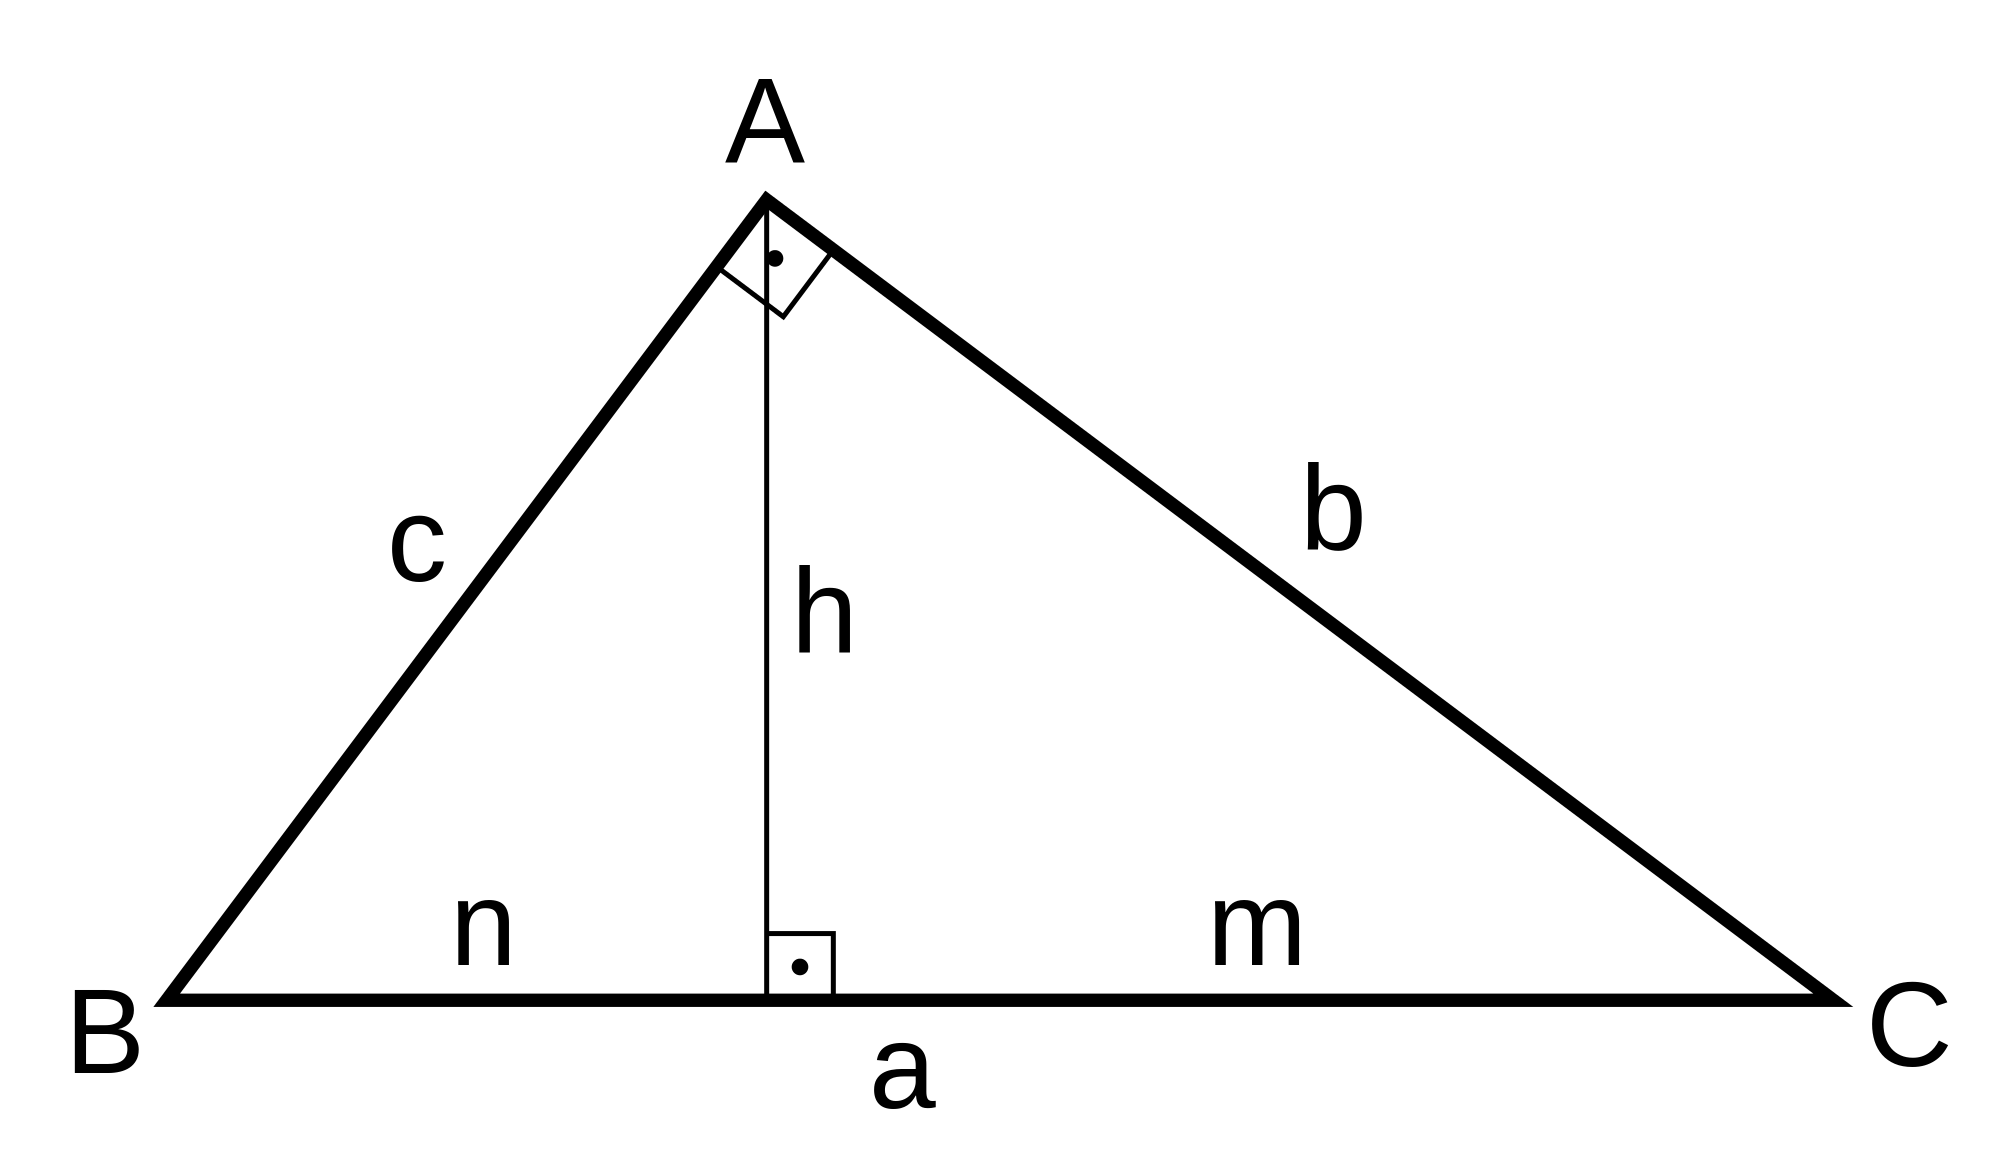
\includegraphics[width=\linewidth]{right_triangle}
  \end{minipage}
\end{figure}

\subsection{Equilateral Triangle}
\[h = \frac{a \sqrt{3}}{2}\]
\[r = \frac{a \sqrt{3}}{6}\]
\[R = \frac{a \sqrt{3}}{3}\]
\[A = \frac{a^2 \sqrt{3}}{4}\]

\subsection{All Triangles}
\[A = a b \sin \gamma \]
\[A = \sqrt{p \left ( p - a \right ) \left ( p - b \right ) \left ( p - c \right )}\]
\[a^2 = b^2 + c^2 - 2 b c \cos \alpha\]
\[\frac{a}{\sin \alpha} = \frac{b}{\sin \beta} = \frac{c}{\sin \gamma} = 2R\]

\section{Equations}
\subsection{Discriminant}
\[\Delta = b^2 - 4ac\]

\subsection{Vieta's formulas}
A polynomial \(P(x) = a_n x^n + a_{n-1} x^{n-1} + ... + a_0\), (with the coefficients being real or complex numbers and \(a_n \neq 0\)) is known by the fundamental theorem of algebra to have \(n\) (not necessarily distinct) complex roots \(x_1, x_2, ..., x_n\).

Vieta's formulas relate the polynomial's coefficients \(a_k\) to signed sums and products of its roots \(x_i\) as follows:

\[\sum_{1 \le i \le n} x_i = - \frac{a_{n-1}}{a_n}\]
\[\sum_{1 \le i_1 < i_2 \le n} x_{i_1} x_{i_2} = \frac{a_{n-2}}{a_n}\]
\[\sum_{1 \le i_1 < i_2 < i_3 \le n} x_{i_1} x_{i_2} x_{i_3} = - \frac{a_{n-3}}{a_n}\]
\[\sum_{1 \le i_1 < i_2 < ... < i_k \le n} x_{i_1} x_{i_2} ... x_{i_k} = (-1)^k \frac{a_{n-k}}{a_n}\]

\end{document}